\documentclass{article}\usepackage[]{graphicx}\usepackage[]{xcolor}
% maxwidth is the original width if it is less than linewidth
% otherwise use linewidth (to make sure the graphics do not exceed the margin)
\makeatletter
\def\maxwidth{ %
  \ifdim\Gin@nat@width>\linewidth
    \linewidth
  \else
    \Gin@nat@width
  \fi
}
\makeatother

\definecolor{fgcolor}{rgb}{0.345, 0.345, 0.345}
\newcommand{\hlnum}[1]{\textcolor[rgb]{0.686,0.059,0.569}{#1}}%
\newcommand{\hlstr}[1]{\textcolor[rgb]{0.192,0.494,0.8}{#1}}%
\newcommand{\hlcom}[1]{\textcolor[rgb]{0.678,0.584,0.686}{\textit{#1}}}%
\newcommand{\hlopt}[1]{\textcolor[rgb]{0,0,0}{#1}}%
\newcommand{\hlstd}[1]{\textcolor[rgb]{0.345,0.345,0.345}{#1}}%
\newcommand{\hlkwa}[1]{\textcolor[rgb]{0.161,0.373,0.58}{\textbf{#1}}}%
\newcommand{\hlkwb}[1]{\textcolor[rgb]{0.69,0.353,0.396}{#1}}%
\newcommand{\hlkwc}[1]{\textcolor[rgb]{0.333,0.667,0.333}{#1}}%
\newcommand{\hlkwd}[1]{\textcolor[rgb]{0.737,0.353,0.396}{\textbf{#1}}}%
\let\hlipl\hlkwb

\usepackage{framed}
\makeatletter
\newenvironment{kframe}{%
 \def\at@end@of@kframe{}%
 \ifinner\ifhmode%
  \def\at@end@of@kframe{\end{minipage}}%
  \begin{minipage}{\columnwidth}%
 \fi\fi%
 \def\FrameCommand##1{\hskip\@totalleftmargin \hskip-\fboxsep
 \colorbox{shadecolor}{##1}\hskip-\fboxsep
     % There is no \\@totalrightmargin, so:
     \hskip-\linewidth \hskip-\@totalleftmargin \hskip\columnwidth}%
 \MakeFramed {\advance\hsize-\width
   \@totalleftmargin\z@ \linewidth\hsize
   \@setminipage}}%
 {\par\unskip\endMakeFramed%
 \at@end@of@kframe}
\makeatother

\definecolor{shadecolor}{rgb}{.97, .97, .97}
\definecolor{messagecolor}{rgb}{0, 0, 0}
\definecolor{warningcolor}{rgb}{1, 0, 1}
\definecolor{errorcolor}{rgb}{1, 0, 0}
\newenvironment{knitrout}{}{} % an empty environment to be redefined in TeX

\usepackage{alltt}
\usepackage[sc]{mathpazo}
\renewcommand{\sfdefault}{lmss}
\renewcommand{\ttdefault}{lmtt}
\usepackage[T1]{fontenc}
\usepackage{geometry}
\geometry{verbose,tmargin=2.5cm,bmargin=2.5cm,lmargin=2.5cm,rmargin=2.5cm}
\setcounter{secnumdepth}{2}
\setcounter{tocdepth}{2}
\usepackage[unicode=true,pdfusetitle,
 bookmarks=true,bookmarksnumbered=true,bookmarksopen=true,bookmarksopenlevel=2,
 breaklinks=false,pdfborder={0 0 1},backref=false,colorlinks=false]
 {hyperref}
\hypersetup{
 pdfstartview={XYZ null null 1}}

\makeatletter
%%%%%%%%%%%%%%%%%%%%%%%%%%%%%% User specified LaTeX commands.
\renewcommand{\textfraction}{0.05}
\renewcommand{\topfraction}{0.8}
\renewcommand{\bottomfraction}{0.8}
\renewcommand{\floatpagefraction}{0.75}

\makeatother
\IfFileExists{upquote.sty}{\usepackage{upquote}}{}
\begin{document}








The results below are generated from an R script.

\begin{knitrout}
\definecolor{shadecolor}{rgb}{0.969, 0.969, 0.969}\color{fgcolor}\begin{kframe}
\begin{alltt}
\hlkwd{setwd}\hlstd{(}\hlstr{'~/Dsc520'}\hlstd{)}
\hlkwd{library}\hlstd{(ggplot2)}
\hlkwd{library}\hlstd{(readr)}
\hlkwd{library}\hlstd{(readxl)}
\hlkwd{library}\hlstd{(dplyr)}
\hlkwd{library}\hlstd{(scales)}
\end{alltt}


{\ttfamily\noindent\itshape\color{messagecolor}{\#\# \\\#\# 载入程辑包:'scales'}}

{\ttfamily\noindent\itshape\color{messagecolor}{\#\# The following object is masked from 'package:readr':\\\#\# \\\#\# \ \ \ \ col\_factor}}\begin{alltt}
\hlstd{source_Url} \hlkwb{<-} \hlstr{"http://content.bellevue.edu/cst/dsc/520/id/resources/10-week-housing-data/week-6-housing.xlsx"}
\hlkwd{download.file}\hlstd{(}\hlkwc{url}\hlstd{=source_Url,} \hlkwc{destfile} \hlstd{=} \hlstr{'data/exercisedata.xlsx'}\hlstd{,} \hlkwc{method}\hlstd{=}\hlstr{'curl'}\hlstd{)}
\hlstd{housing} \hlkwb{<-} \hlkwd{read_excel}\hlstd{(}\hlstr{'data/exercisedata.xlsx'}\hlstd{)}
\hlcom{#head(housing)}
\hlcom{#str(housing)}
\hlstd{Sale_price} \hlkwb{=} \hlkwd{select}\hlstd{(housing, `Sale Price`)}
\hlstd{Total_Sale_Price} \hlkwb{<-} \hlkwd{apply}\hlstd{(Sale_price,} \hlnum{2}\hlstd{, sum)}

\hlstd{Zipcode_SalePrice_mean} \hlkwb{<-} \hlkwd{aggregate}\hlstd{(`Sale Price`} \hlopt{~} \hlstd{zip5,} \hlkwc{data} \hlstd{= housing, mean)}
\hlstd{Zipcode_SalePrice_mean}
\end{alltt}
\begin{verbatim}
##    zip5 Sale Price
## 1 98052   649375.4
## 2 98053   672623.7
## 3 98059   645000.0
## 4 98074   951543.8
\end{verbatim}
\begin{alltt}
\hlstd{housing_by_zip} \hlkwb{<-} \hlstd{housing} \hlopt \hlkwd{group_by}\hlstd{(zip5)}
\hlkwd{View}\hlstd{(housing_by_zip)}
\hlstd{Count_by_Sales} \hlkwb{<-} \hlkwd{summarize}\hlstd{(housing_by_zip,} \hlkwc{Count_of_Sales} \hlstd{=} \hlkwd{n}\hlstd{())}
\hlkwd{View}\hlstd{(Count_by_Sales)}
\hlstd{Housing_by_zip_bedroom} \hlkwb{<-} \hlkwd{group_by}\hlstd{(housing, zip5, bedrooms)}
\hlkwd{View}\hlstd{(Housing_by_zip_bedroom)}
\hlstd{Count_by_sales_room} \hlkwb{<-} \hlkwd{summarize}\hlstd{(Housing_by_zip_bedroom,} \hlkwc{count} \hlstd{=} \hlkwd{n}\hlstd{())}
\end{alltt}


{\ttfamily\noindent\itshape\color{messagecolor}{\#\# `summarise()` has grouped output by 'zip5'. You can override using the `.groups`\\\#\# argument.}}\begin{alltt}
\hlkwd{View}\hlstd{(Count_by_sales_room)}
\hlstd{Count_by_sales_room_avg} \hlkwb{<-}\hlkwd{summarize}\hlstd{(Housing_by_zip_bedroom,}
                                    \hlkwc{avg_price} \hlstd{=} \hlkwd{mean}\hlstd{(`Sale Price`))}
\end{alltt}


{\ttfamily\noindent\itshape\color{messagecolor}{\#\# `summarise()` has grouped output by 'zip5'. You can override using the `.groups`\\\#\# argument.}}\begin{alltt}
\hlkwd{View}\hlstd{(Count_by_sales_room_avg)}

\hlkwd{options}\hlstd{(}\hlkwc{scipen} \hlstd{=} \hlnum{999}\hlstd{)}
\hlkwd{ggplot}\hlstd{(housing,} \hlkwd{aes}\hlstd{(}\hlkwc{x}\hlstd{=`Sale Price`))} \hlopt{+}\hlkwd{geom_histogram}\hlstd{()} \hlopt{+}\hlkwd{facet_wrap}\hlstd{(}\hlopt{~}\hlstd{bedrooms)}\hlopt{+}
\hlkwd{ggtitle}\hlstd{(}\hlstr{"Sales Historgram per beedroom"}\hlstd{)} \hlopt{+} \hlkwd{xlab}\hlstd{(}\hlstr{"Bedrooms"}\hlstd{)} \hlopt{+}\hlkwd{ylab}\hlstd{(}\hlstr{"Sale Price"}\hlstd{)}
\end{alltt}


{\ttfamily\noindent\itshape\color{messagecolor}{\#\# `stat\_bin()` using `bins = 30`. Pick better value with `binwidth`.}}\end{kframe}

{\centering 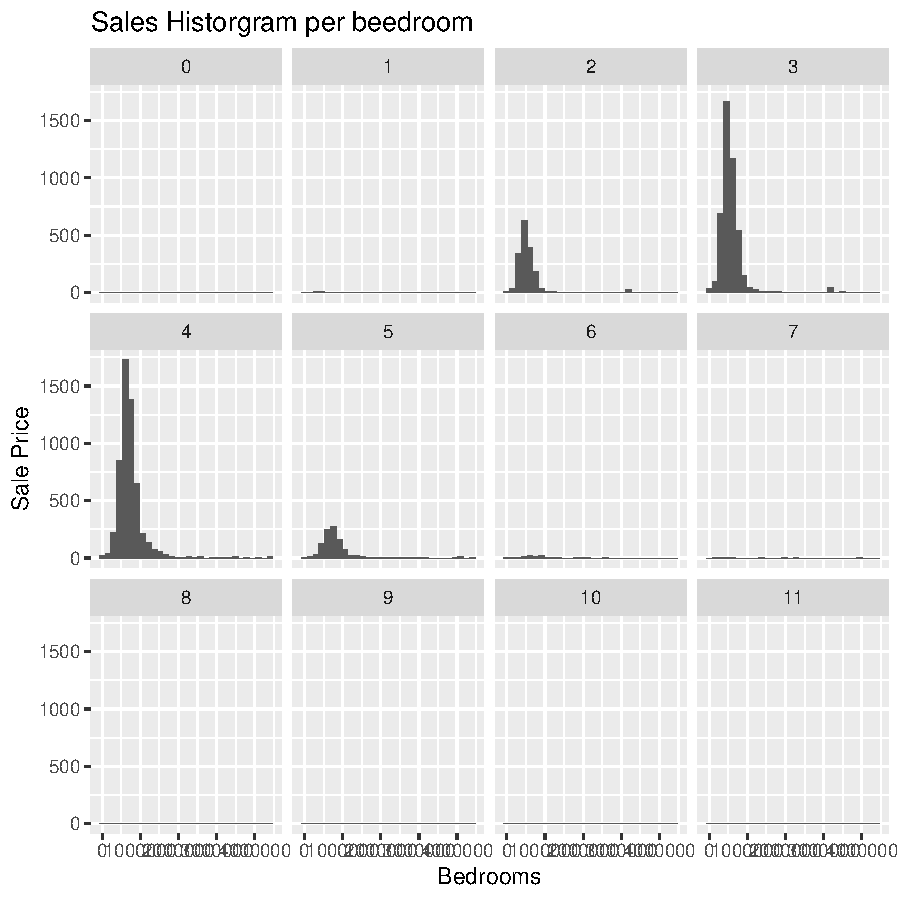
\includegraphics[width=.6\linewidth]{figure/DSC520-week4-housing-TangXin-Rnwauto-report-1} 

}


\begin{kframe}\begin{alltt}
\hlkwd{ggplot}\hlstd{(housing,} \hlkwd{aes}\hlstd{(}\hlkwc{x}\hlstd{=bedrooms,} \hlkwc{y}\hlstd{=`Sale Price`))} \hlopt{+} \hlkwd{geom_point}\hlstd{()} \hlopt{+} \hlkwd{scale_y_continuous}\hlstd{(}\hlkwc{labels} \hlstd{=} \hlkwd{label_number}\hlstd{(}\hlkwc{scale_cut} \hlstd{=} \hlkwd{cut_short_scale}\hlstd{()))}
\end{alltt}
\end{kframe}

{\centering 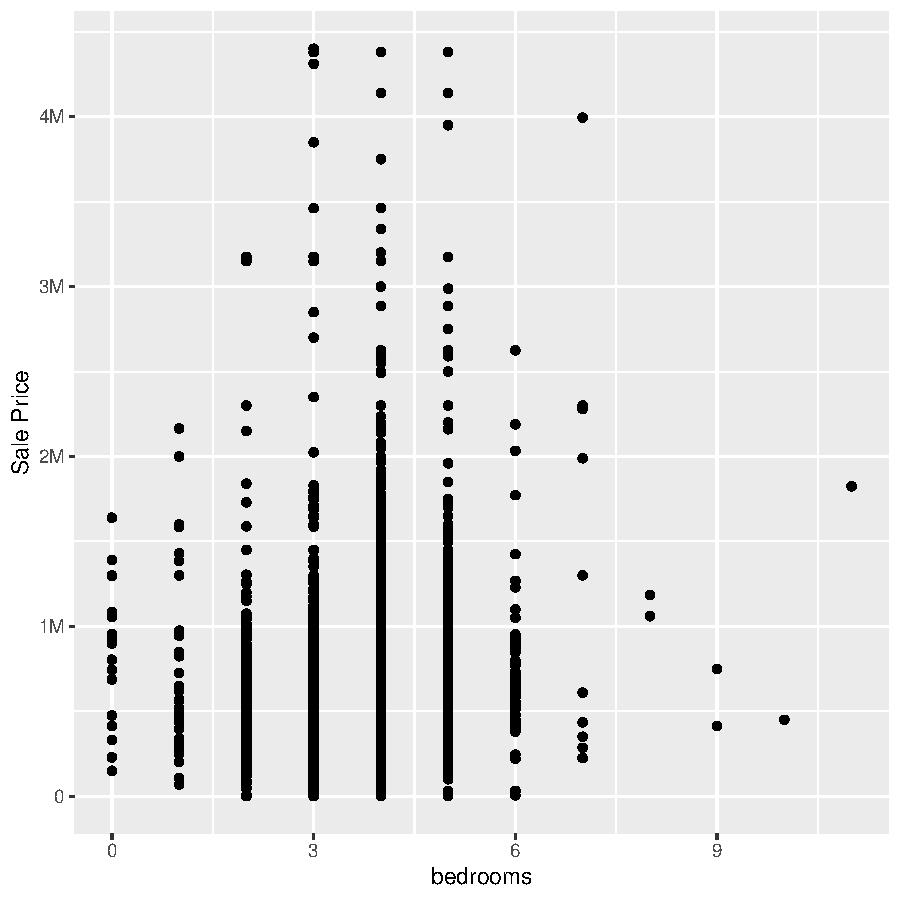
\includegraphics[width=.6\linewidth]{figure/DSC520-week4-housing-TangXin-Rnwauto-report-2} 

}


\begin{kframe}\begin{alltt}
\hlkwd{ggplot}\hlstd{(housing,} \hlkwd{aes}\hlstd{(}\hlkwc{x}\hlstd{=`Sale Price`))} \hlopt{+}\hlkwd{geom_histogram}\hlstd{()} \hlopt{+} \hlkwd{scale_y_continuous}\hlstd{(}\hlkwc{labels} \hlstd{=} \hlkwd{label_number}\hlstd{(}\hlkwc{scale_cut} \hlstd{=} \hlkwd{cut_short_scale}\hlstd{()))}
\end{alltt}


{\ttfamily\noindent\itshape\color{messagecolor}{\#\# `stat\_bin()` using `bins = 30`. Pick better value with `binwidth`.}}\end{kframe}

{\centering 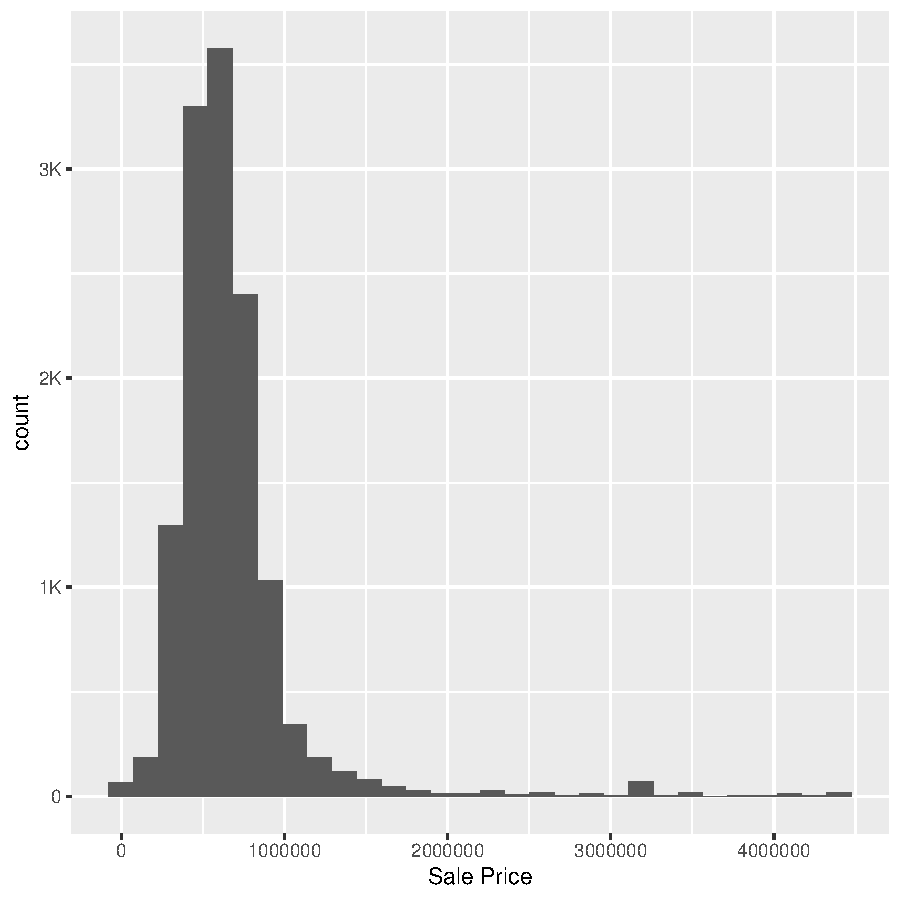
\includegraphics[width=.6\linewidth]{figure/DSC520-week4-housing-TangXin-Rnwauto-report-3} 

}


\end{knitrout}

The R session information (including the OS info, R version and all
packages used):

\begin{knitrout}
\definecolor{shadecolor}{rgb}{0.969, 0.969, 0.969}\color{fgcolor}\begin{kframe}
\begin{alltt}
\hlkwd{sessionInfo}\hlstd{()}
\end{alltt}
\begin{verbatim}
## R version 4.3.1 (2023-06-16 ucrt)
## Platform: x86_64-w64-mingw32/x64 (64-bit)
## Running under: Windows 10 x64 (build 19045)
## 
## Matrix products: default
## 
## 
## locale:
## [1] LC_COLLATE=English_United States.utf8  LC_CTYPE=English_United States.utf8   
## [3] LC_MONETARY=English_United States.utf8 LC_NUMERIC=C                          
## [5] LC_TIME=English_United States.utf8    
## 
## time zone: America/Chicago
## tzcode source: internal
## 
## attached base packages:
## [1] stats     graphics  grDevices utils     datasets  methods   base     
## 
## other attached packages:
## [1] scales_1.2.1  readxl_1.4.2  readr_2.1.4   ggplot2_3.4.2 tinytex_0.45  dplyr_1.1.2  
## 
## loaded via a namespace (and not attached):
##  [1] vctrs_0.6.2      cli_3.6.1        knitr_1.43       rlang_1.1.1      xfun_0.39       
##  [6] highr_0.10       generics_0.1.3   labeling_0.4.2   glue_1.6.2       colorspace_2.1-0
## [11] hms_1.1.3        fansi_1.0.4      cellranger_1.1.0 grid_4.3.1       evaluate_0.21   
## [16] munsell_0.5.0    tibble_3.2.1     tzdb_0.4.0       lifecycle_1.0.3  compiler_4.3.1  
## [21] pkgconfig_2.0.3  rstudioapi_0.14  farver_2.1.1     R6_2.5.1         tidyselect_1.2.0
## [26] utf8_1.2.3       pillar_1.9.0     magrittr_2.0.3   tools_4.3.1      withr_2.5.0     
## [31] gtable_0.3.3
\end{verbatim}
\begin{alltt}
\hlkwd{Sys.time}\hlstd{()}
\end{alltt}
\begin{verbatim}
## [1] "2023-06-29 18:01:45 CDT"
\end{verbatim}
\end{kframe}
\end{knitrout}


\end{document}
